\begin{frame}{Path merged : thread 2}
    \setbeamercovered{invisible}
\RaggedRight
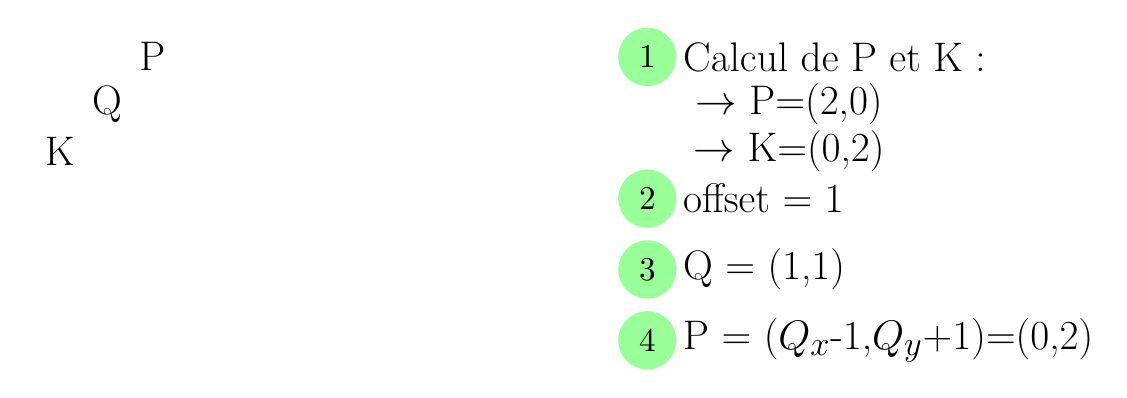
\begin{tikzpicture}[line cap=round,scale=0.6, every node/.style={transform shape}]
    \baseGraph
    \maze (-3,6) node {\BlueRoute}--(-3,5)node {\BlueRoute};
    \maze (-3,5) node {\BlueRoute}--(-3,4)node {\BlueRoute}; %ajouter ce qu'on a déjà fait 
    \draw (10,6) node[shape = circle,label=right:\Huge{Calcul de P et K :},fill=green!40,scale=2] {1};\pause 
    \draw (13,5) node {\Huge{$\rightarrow$ P=(2,0)}}; 
    \draw (-1,6) node[label=right:\Huge{P}] {\BlackCirc};\pause
    \draw (13,4) node {\Huge{$\rightarrow$ K=(0,2)}};
    \draw (-3,4) node[label=right:\Huge{K}] {\BlackCirc};\pause
    \draw (10,3) node[shape = circle,label=right:\Huge{offset = 1},fill=green!40,scale=2] {2};\pause
    \draw (10,1.5) node[shape = circle,label=right:\Huge{Q = (1,1)},fill=green!40,scale=2] {3};
    \draw (-2,5) node[label=right:\Huge{Q}] {\BlackCirc};\pause
    \draw (10,0) node[shape = circle,label=right:\Huge{P = ($Q_{x}$-1,$Q_{y}$+1)=(0,2)},fill=green!40,scale=2] {4};\pause 
    %\draw (10,-1.5) node[shape = circle,label=right:\Huge{M[i]=A[$Q_{y}$]},fill=green!40,scale=2] {5}; 
    %\draw (-3,6) node {\BlueRoute}; \pause
\end{tikzpicture}
\end{frame}



\begin{frame}{Path merged : thread 2}
    \setbeamercovered{invisible}
\RaggedRight
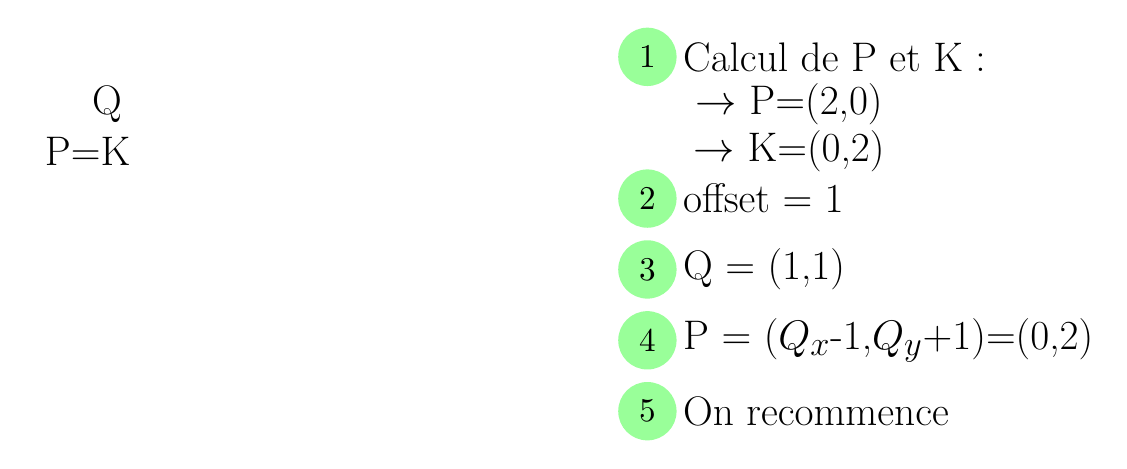
\begin{tikzpicture}[line cap=round,scale=0.6, every node/.style={transform shape}]
    \baseGraph
    \maze (-3,6) node {\BlueRoute}--(-3,5)node {\BlueRoute};
    \maze (-3,5) node {\BlueRoute}--(-3,4)node {\BlueRoute}; %ajouter ce qu'on a déjà fait 
    \draw (10,6) node[shape = circle,label=right:\Huge{Calcul de P et K :},fill=green!40,scale=2] {1}; 
    \draw (13,5) node {\Huge{$\rightarrow$ P=(2,0)}}; 
    \draw (-3,4) node[label=right:\Huge{P=K}] {\BlackCirc};
    \draw (13,4) node {\Huge{$\rightarrow$ K=(0,2)}};
    \draw (10,3) node[shape = circle,label=right:\Huge{offset = 1},fill=green!40,scale=2] {2};
    \draw (10,1.5) node[shape = circle,label=right:\Huge{Q = (1,1)},fill=green!40,scale=2] {3};
    \draw (-2,5) node[label=right:\Huge{Q}] {\BlackCirc};
    \draw (10,0) node[shape = circle,label=right:\Huge{P = ($Q_{x}$-1,$Q_{y}$+1)=(0,2)},fill=green!40,scale=2] {4};\pause 
    \draw (10,-1.5) node[shape = circle,label=right:\Huge{On recommence},fill=green!40,scale=2] {5}; 
    %\draw (-3,6) node {\BlueRoute}; \pause
\end{tikzpicture}
\end{frame}
\begin{frame}{Path merged : thread 2}
    \setbeamercovered{invisible}
\RaggedRight
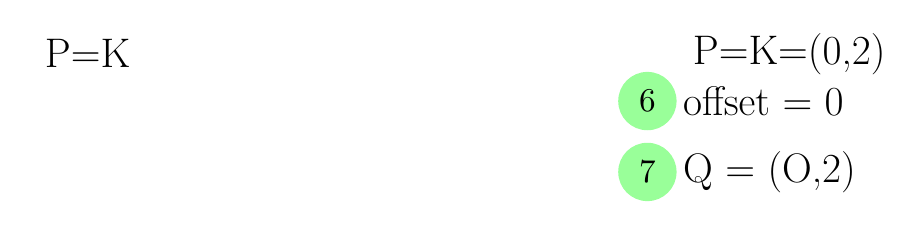
\begin{tikzpicture}[line cap=round,scale=0.6, every node/.style={transform shape}]
    \baseGraph
    \maze (-3,6) node {\BlueRoute}--(-3,5)node {\BlueRoute};
    \maze (-3,5) node {\BlueRoute}--(-3,4)node {\BlueRoute}; %ajouter ce qu'on a déjà fait 
 
    \draw (-3,4) node[label=right:\Huge{P=K}] {\BlackCirc};
    \draw (13,4) node {\Huge{P=K=(0,2)}};
    \draw (10,3) node[shape = circle,label=right:\Huge{offset = 0},fill=green!40,scale=2] {6};\pause
    \draw (10,1.5) node[shape = circle,label=right:\Huge{Q = (O,2)},fill=green!40,scale=2] {7};
\end{tikzpicture}
\end{frame}


\begin{frame}{Path merged : thread 2}
    \setbeamercovered{invisible}
\RaggedRight
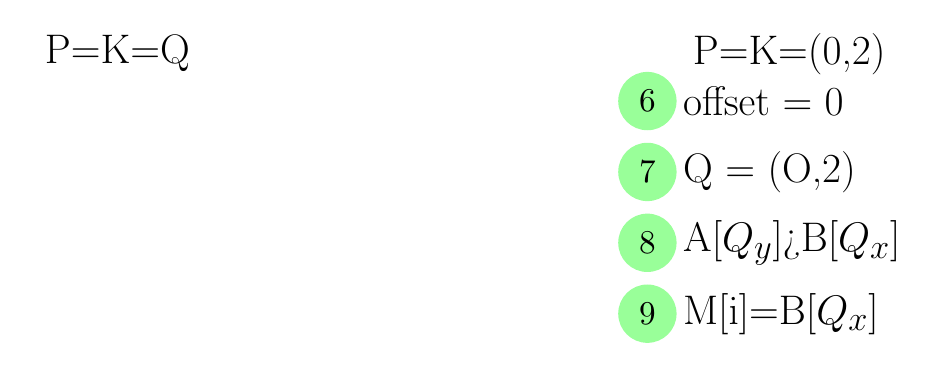
\begin{tikzpicture}[line cap=round,scale=0.6, every node/.style={transform shape}]
    \baseGraph
    \maze (-3,6) node {\BlueRoute}--(-3,5)node {\BlueRoute};
    \maze (-3,5) node {\BlueRoute}--(-3,4)node {\BlueRoute}; %ajouter ce qu'on a déjà fait 
 
    \draw (-3,4) node[label=right:\Huge{P=K=Q}] {\BlackCirc};
    \draw (13,4) node {\Huge{P=K=(0,2)}};
    \draw (10,3) node[shape = circle,label=right:\Huge{offset = 0},fill=green!40,scale=2] {6};
    \draw (10,1.5) node[shape = circle,label=right:\Huge{Q = (O,2)},fill=green!40,scale=2] {7};
    \draw (10,0) node[shape = circle,label=right:\Huge{A[$Q_{y}$]>B[$Q_{x}$]},fill=green!40,scale=2] {8};\pause 
    \draw (10,-1.5) node[shape = circle,label=right:\Huge{M[i]=B[$Q_{x}$]},fill=green!40,scale=2] {9}; 
\end{tikzpicture}
\end{frame}



\begin{frame}{Path merged : thread 2, path}
    \setbeamercovered{invisible}
\RaggedRight
\begin{tikzpicture}[line cap=round,scale=0.6, every node/.style={transform shape}]
    \baseGraph
    \draw (-3,6) node {\BlueRoute}; 
    \maze (-3,6) node {\BlueRoute}--(-3,5)node {\BlueRoute};
    \maze (-3,5) node {\BlueRoute}--(-3,4)node {\BlueRoute};\pause
    \maze (-3,4) node {\BlueRoute}--(-2,4)node {\BlueRoute};
\end{tikzpicture}
\end{frame}